\chapter{Software}
Die Software, die verwendet wird, teilt sich in 5 Teile auf:
\begin{itemize}
\item Auslesen der Sensoren, Aufbereiten der Daten und allgemeine Steuerung (main.sh)
\item Steuern des Displays
\item Webinterface (Livedaten, grafische Darstellung und Informationen)
\item mathematische Endauswertung
\item sonstiges
\end{itemize}

\section{main.sh}
\label{sec:main.sh}

Das wichtigste Programm ist das \gls{Bash}-Script \textit{main.sh}. Mithilfe eines solchen können Programme gesteuert und ihre Ausgaben verarbeitet werden. Dieses Script kümmert sich um die Aufzeichnung, erste Verarbeitung und Speicherung der Daten und die Steuerung der anderen Programme. 

\subsection{Allgemeines}
\label{subsec:main.sh/allgemeines}

Zunächst werden die Pins angegeben, an denen die \gls{LED}s angeschlossen sind. In den Zeilen 11-13 wird nun die grüne \gls{LED} eingeschaltet, um zu zeigen, dass das Programm läuft.
\code{main.sh}{bash}{8}{13}

Nun startet das eigentliche Programm. Alles, was nun folgt wird wiederholt, bis die Aufzeichnung beendet wird.
\code{main.sh}{bash}{27}{28}
In den folgenden drei Zeilen wird der aktuelle Zeitpunkt in drei verschiedenen Formaten für drei verschiedene Zwecke gespeichert.
\begin{table}[h]
	\centering
	\begin{tabulary}{\textwidth}{C|C|C}
		Code & Beispiel & Verwendung \\
		\hline
		\hline
		\%Y/\%m/\%d\ \%H:\%M:\%S & 2014/11/23 16:47:50 & Format zum Abspeichern in \gls{CSV} \\
		\hline
		\%d.\%m\ \%H:\%M:\%S & 23.11 16:47:50 & einfach lesbares Format für das Display \\
		\hline
		\%d.\%m.\%y\ \%H:\%M:\%S & 23.11.2014 16:47:50 & einfaches, exaktes Format für das Webinterface \\
	\end{tabulary}
	\caption{Datumsformate}
\end{table}

\code{main.sh}{bash}{29}{31}

\subsection{Messung}
\label{subsec:main.sh/messung}

Als erstes werden die Sensoren ausgelesen. Am einfachsten kann mit dem im Raspberry Pi integrierten Thermometer die \gls{CPU}-Temperatur ausgelesen werden. Hierzu muss\todo{müssen?} nur eine \gls{Geraetedatei} geöffnet und daraus die Zeichen 6-9 gelesen werden:
\codeline{main.sh}{bash}{32}

Nur wenig aufwändiger sind die Temperatursensoren (\emph{DS18B20}, siehe \ref{subsec:Temperatur}). Da die Sensoren manchmal ungültige Werte zurückgeben, wird nach der ersten Messung überprüft, ob dies der Fall ist (Zeile 34) und die Messung solange wiederholt, bis eine gültige Messung erfolgt.
\code{main.sh}{bash}{33}{40}

Die Adafruit-Programme\footcite{DHT}\footcite{bmp058_adafruit}, die den Luftfeuchtesensor (siehe \ref{subsec:Luftfeuchtigkeit}) und den Luftdrucksensor (siehe \ref{subsec:Luftdruck}) auslesen, geben die Feuchtigkeit und die Temperatur durch einen Strichpunkt getrennt an. Daher wird dies zu Beginn als Trennzeichen angegeben. 
\codeline{main.sh}{bash}{4}
Dadurch kann die Ausgabe einfach aufgetrennt werden:
\code{main.sh}{bash}{66}{69}
Auch hier wird bei ungültigen Messwerten mehrmals gemessen.

Der relative Wert für die Luftqualität wird direkt von \emph{usb-sensors-linux}\footcite{usb-sensors-linux} zurückgegeben und muss daher nicht weiterbearbeitet werden.
\codeline{main.sh}{bash}{84}

\subsection{Speichern, Aufbereiten und Verarbeiten}

Nachdem alle Sensoren ausgelesen wurden, müssen sie dauerhaft gespeichert werden. Hierzu werden alle Werte durch ein Komma getrennt und als neue Zeile an die bisherigen Messungen angehängt.
\code{main.sh}{bash}{89}{90}
Hierdurch entsteht eine \gls{CSV}-Datei die wie folgt aussehen kann:
\dateiklein{dygraphs.csv}
Diese Datei wird in den Ordner des Webservers kopiert, damit sie grafisch dargestellt werden kann (siehe \ref{subsec:Diagramme}). Weiters verwendet die \textit{Endauswertung} (siehe \ref{sec:Endauswertung}) auch diese Datei zur rechnerischen Auswertung.

Als nächstes wird der Text für das Display (siehe \ref{sec:Display}) erzeugt. Da dort der Platz beschränkt ist (16x2 Zeichen), werden alle Messwerte um 3 Stellen (bzw. 2 bei Luftdruck) gekürzt. Anschließend werden diese Daten in \emph{text.txt} (für Display) und \emph{text\_ws.txt} (für Webinterface) exportiert.
\codeline{main.sh}{bash}{92}
\datei{text.txt}
\lstinputlisting[style=mystyle,label=textws.txt,caption=text\_ws.txt,basicstyle=\footnotesize]{code/text_ws.txt}

Abschließend wird noch 8 Sekunden gewartet und jedes tausende Mal ein Backup gemacht und mir per E-Mail geschickt, bevor die nächste Messung von vorne beginnt.

\section{Display}
\label{sec:Software/Display}
Um die aktuellen Messungen auch ohne Computer zu sehen, werden sie auch direkt am Raspberry Pi auf einem Display angezeigt (siehe auch \ref{sec:Display}). Um das Display anzusteuern wird ein Programm\footcite{schnatterente_code} von \emph{schnatterente.net} verwendet. Dieses wurde von mir um einige Funktionen ergänzt. 

Das Programm liest aus \emph{text.txt} (siehe Datei \ref{file:text.txt}) die aktuellen Messwerte aus. Da der Platz jedoch stark beschränkt ist, werden diese auf 11 Seiten aufgeteilt, zwischen denen das Display alle 3 Sekunden wechselt.
\begin{figure}[h]
  \centering
     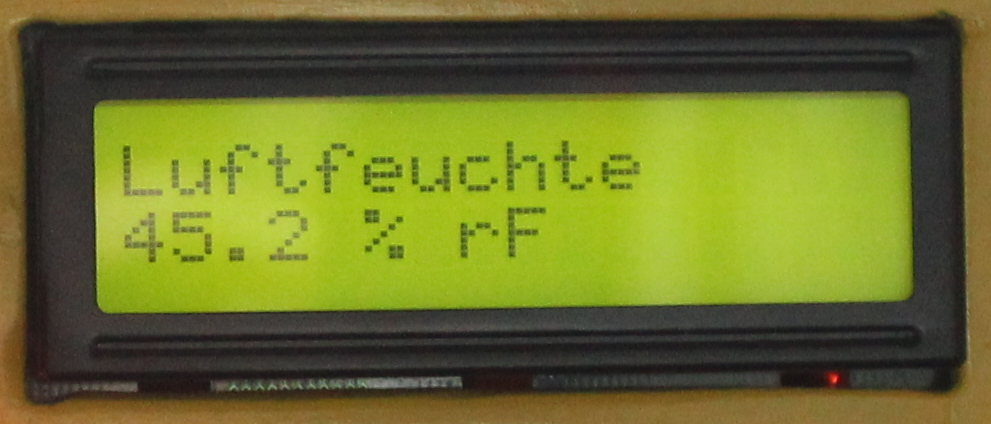
\includegraphics[width=0.9\textwidth]{figures/display.jpg}
  \caption{eingebautes Display (eigenes Werk)}
  \label{fig:display_alt}
\end{figure}

\section{Webinterface}
\label{sec:Webinterface}

Einer der wichtigsten Teile des Projektes ist die grafische Auswertung. Diese kann live auf der Webseite des Raspberry Pi und zeitverzögert unter \href{http://winkler.kremszeile.at}{winkler.kremszeile.at} angesehen werden. Die Auswertung besteht aus zwei von einander unabhängigen Teilen. Zum einen gibt es die Anzeige der Live-Daten, zum anderen die Darstellung der kompletten Aufzeichnung als interaktives Diagramm. Zusätzlich werden auf zwei zusätzlichen Seiten Informationen über das Projekt und Links zu mehr Informationen (siehe Anhang \ref{anhang:weitere_informationen} angezeigt.

\subsection{Livedaten}
\label{subsec:Livedaten}

\begin{figure}[h]
  \centering
     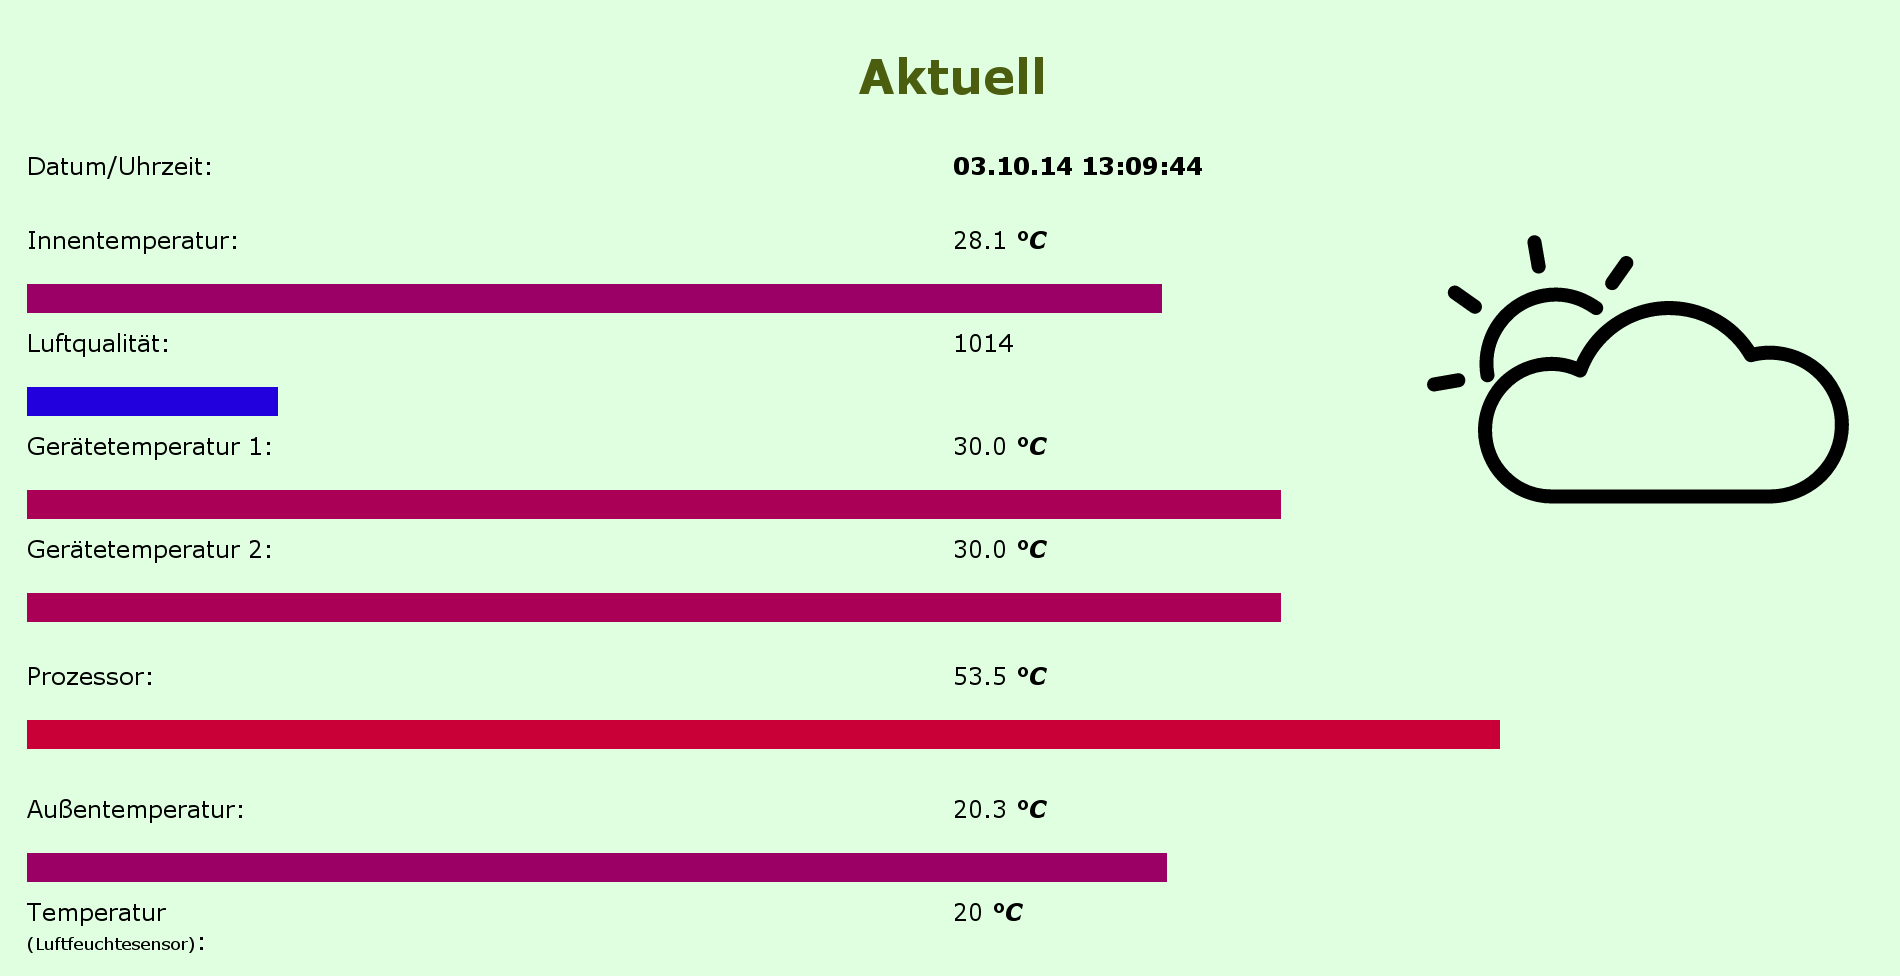
\includegraphics[width=\textwidth]{figures/aktuell.png}
  \caption{Livedaten (Screenshot von \href{http://winkler.kremszeile.at/aktuell.html}{winkler.kremszeile.at/aktuell.html})}
  \label{fig:display_neu}
\end{figure}

Auf Webinterface können die aktuellen Messwerte angezeigt und grafisch veranschaulicht werden.\footnote{\href{http://winkler.kremszeile.at/aktuell.html}{winkler.kremszeile.at/aktuell.html}}
Hierzu wird alle 5 Sekunden mithilfe von \gls{Javascript} die Datei \emph{text\_ws.txt} nachgeladen und ausgewertet. Zusätzlich zur Anzeige der Zahlenwerte werden die Messungen mithilfe von Balken und Farbverläufen angezeigt. Für ältere Webbrowser gibt es auch eine einfache tabellarische Ansicht\footnote{\href{http://winkler.kremszeile.at/aktuell_einfach.html}{winkler.kremszeile.at/aktuell\_einfach.html}}

\subsubsection{Wetter-Rater}
\label{subsubsec:Wetterrater}

Um die Daten auch anders zu nutzen habe ich einen \emph{Wetter-Rater} programmiert. Dieser versucht auf Basis von einfachen Berechnungen und Schätzungen das aktuelle Wetter zu \enquote{erraten}. So wird zum Beispiel die aktuelle Außentemperatur mit der nach Jahreszeit und Tageszeit zu erwartenden Temperatur verglichen, um Rückschlüsse auf den Bewölkungsgrad zu ziehen oder aufgrund der Luftfeuchtigkeit ermittelt, ob es Niederschlag gibt.

Hierzu wird die Temperaturschwankung über einen Tag als Cosinusfunktion mit einer Schwankung von \SI{5}{\degreeCelsius} angenommen.
$$ \textit{Temperaturerwartung} = -5 \cdot \cos\left(\frac{\text{Stunde}\cdot 2 \cdot \pi }{24}\right) + \textit{Mittlere Temp. des Tages}; $$
\begin{figure}[h]
\centering
\begin{tikzpicture}[line cap=round,line join=round,>=triangle 45,x=0.3cm,y=0.5cm]
\draw[->,color=black] (0.,13.) -- (0.,27.);
\draw[color=black] (0.3,27) node [anchor=west] {Temperatur};
\foreach \y in {14,16,18,20,22,24,26}
\draw[shift={(0,\y)},color=black] (2pt,0pt) -- (-2pt,0pt) node[left] {\footnotesize $\y$};

\draw[color=black] (28,18) node [anchor=east] {Stunden};
\draw[->,color=black] (-2.,17.) -- (25.,17.);
\foreach \x in {,5,10,15,20}
\draw[shift={(\x,17)},color=black] (0pt,2pt) -- (0pt,-2pt) node[below] {\footnotesize $\x$};

\clip(-2.,13.) rectangle (25.,27.);
\draw[smooth,samples=100,domain=-2.0:25.0] plot(\x,{0-5.0*cos(((\x)*2.0*3.1415926535/24.0)*180/pi)+20.0});
\end{tikzpicture}
\caption{Graph der Funktion bei mittlere Temp. = \SI{20}{\degreeCelsius} (eigenes Werk)}
\end{figure}


Der Wetter-Rater gibt drei Werte aus:
\begin{itemize}
	\item Tag oder Nacht
	\item Niederschlag (keiner/Gewitter/Schnee/Regen/Schneeregen)
	\item Bewölkungsgrad (sonnig/leicht bewölkt/stark bewölkt)
\end{itemize}
Aufgrund von diesen Werten wird dann eine Grafik (siehe Abbildung \ref{fig:wettericons}) ausgewählt, welche dann angezeigt wird.

\begin{figure}
  \centering
     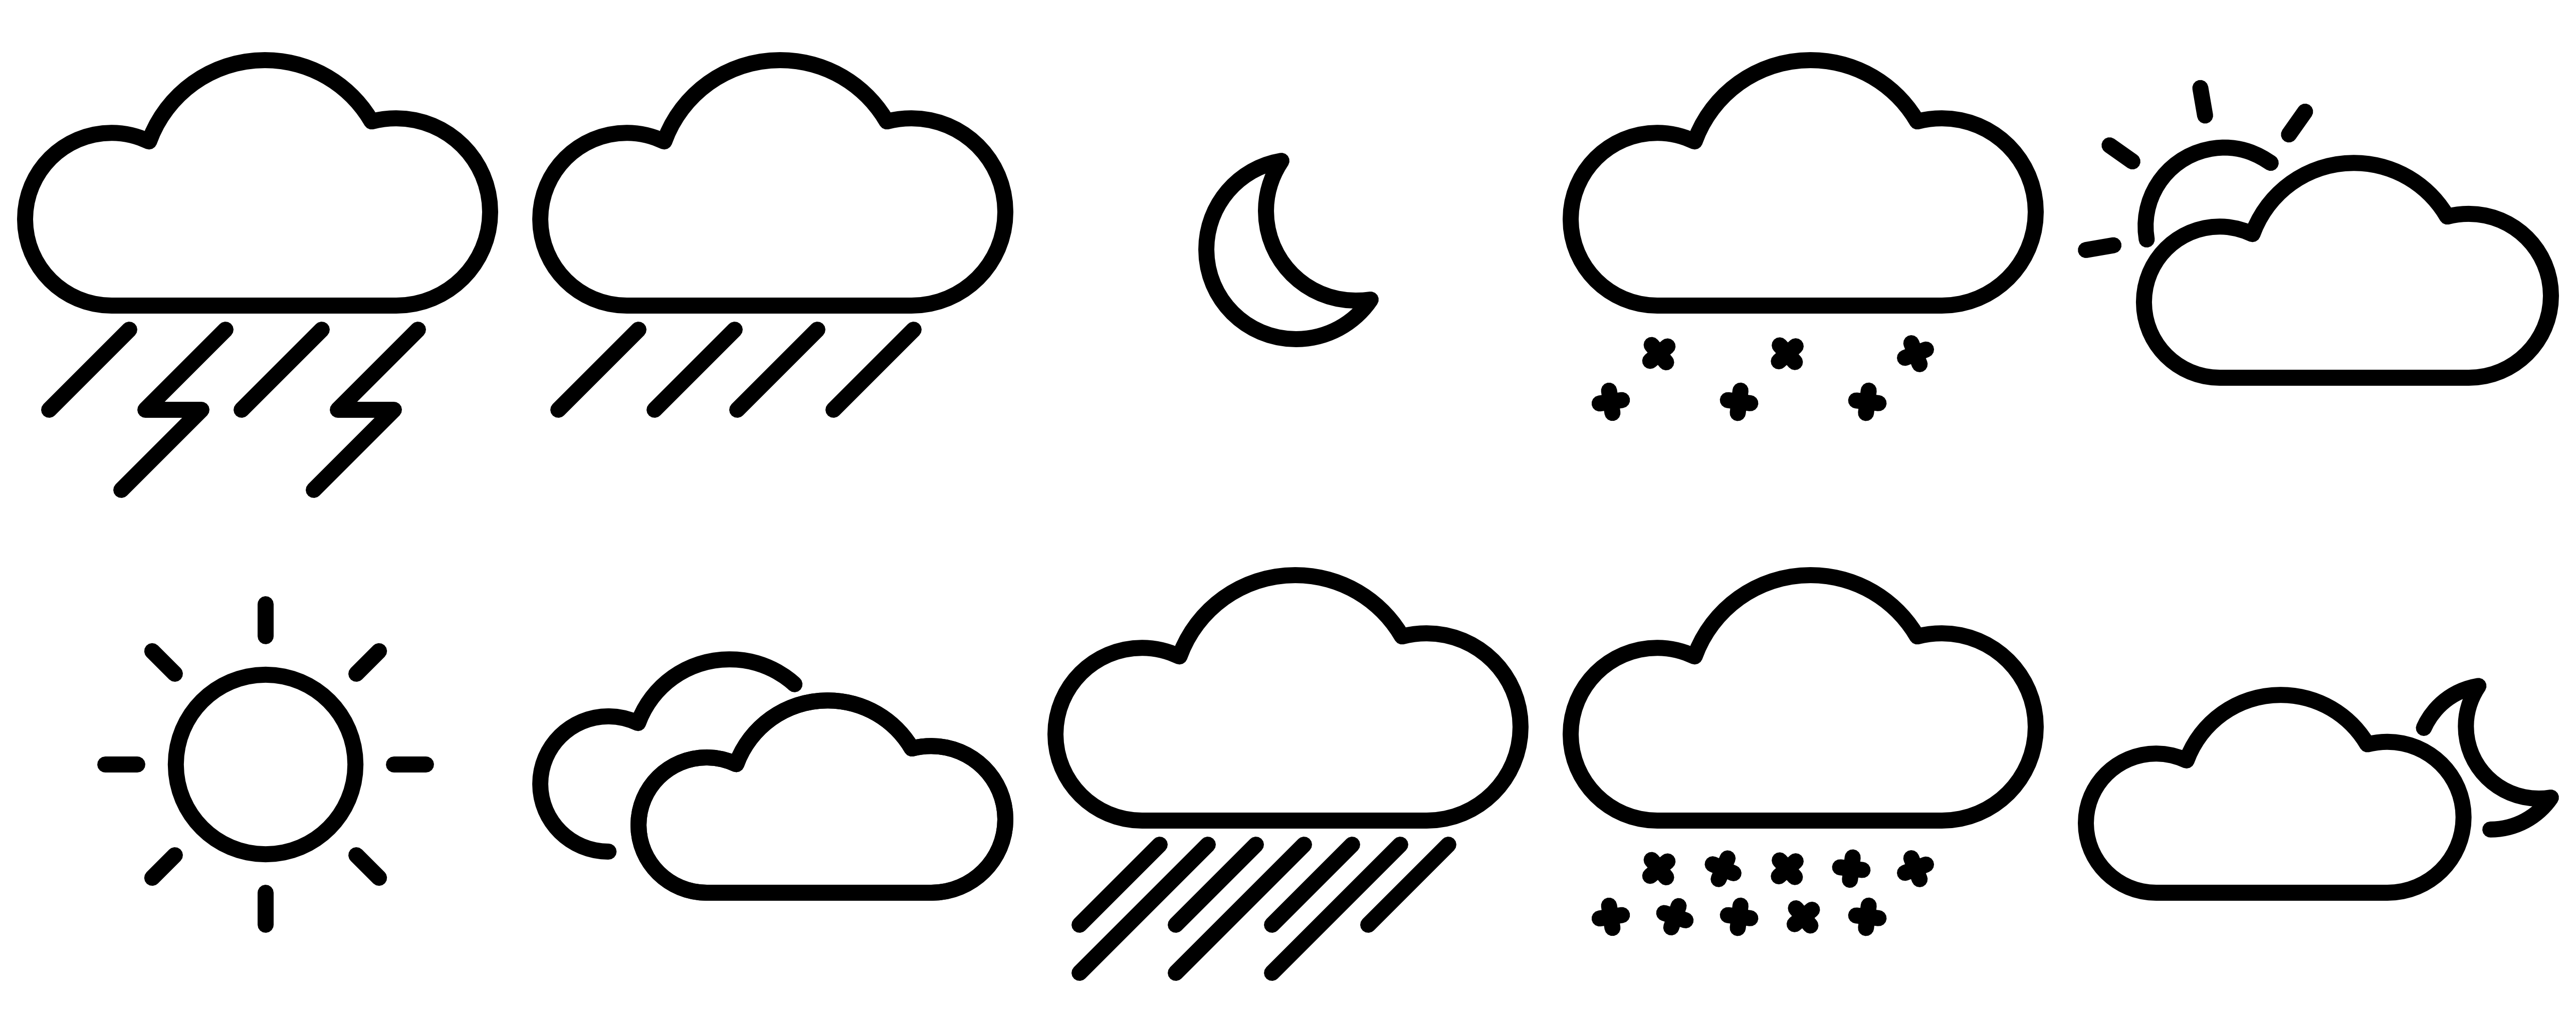
\includegraphics[width=\textwidth]{figures/wettericons.png}
  \caption{Wettericons (eigenes Werk)}
  \label{fig:wettericons}
\end{figure}

\subsection{Diagramme}
\label{subsec:Diagramme}

\begin{figure}[h]
  \centering
     \makebox[\textwidth][c]{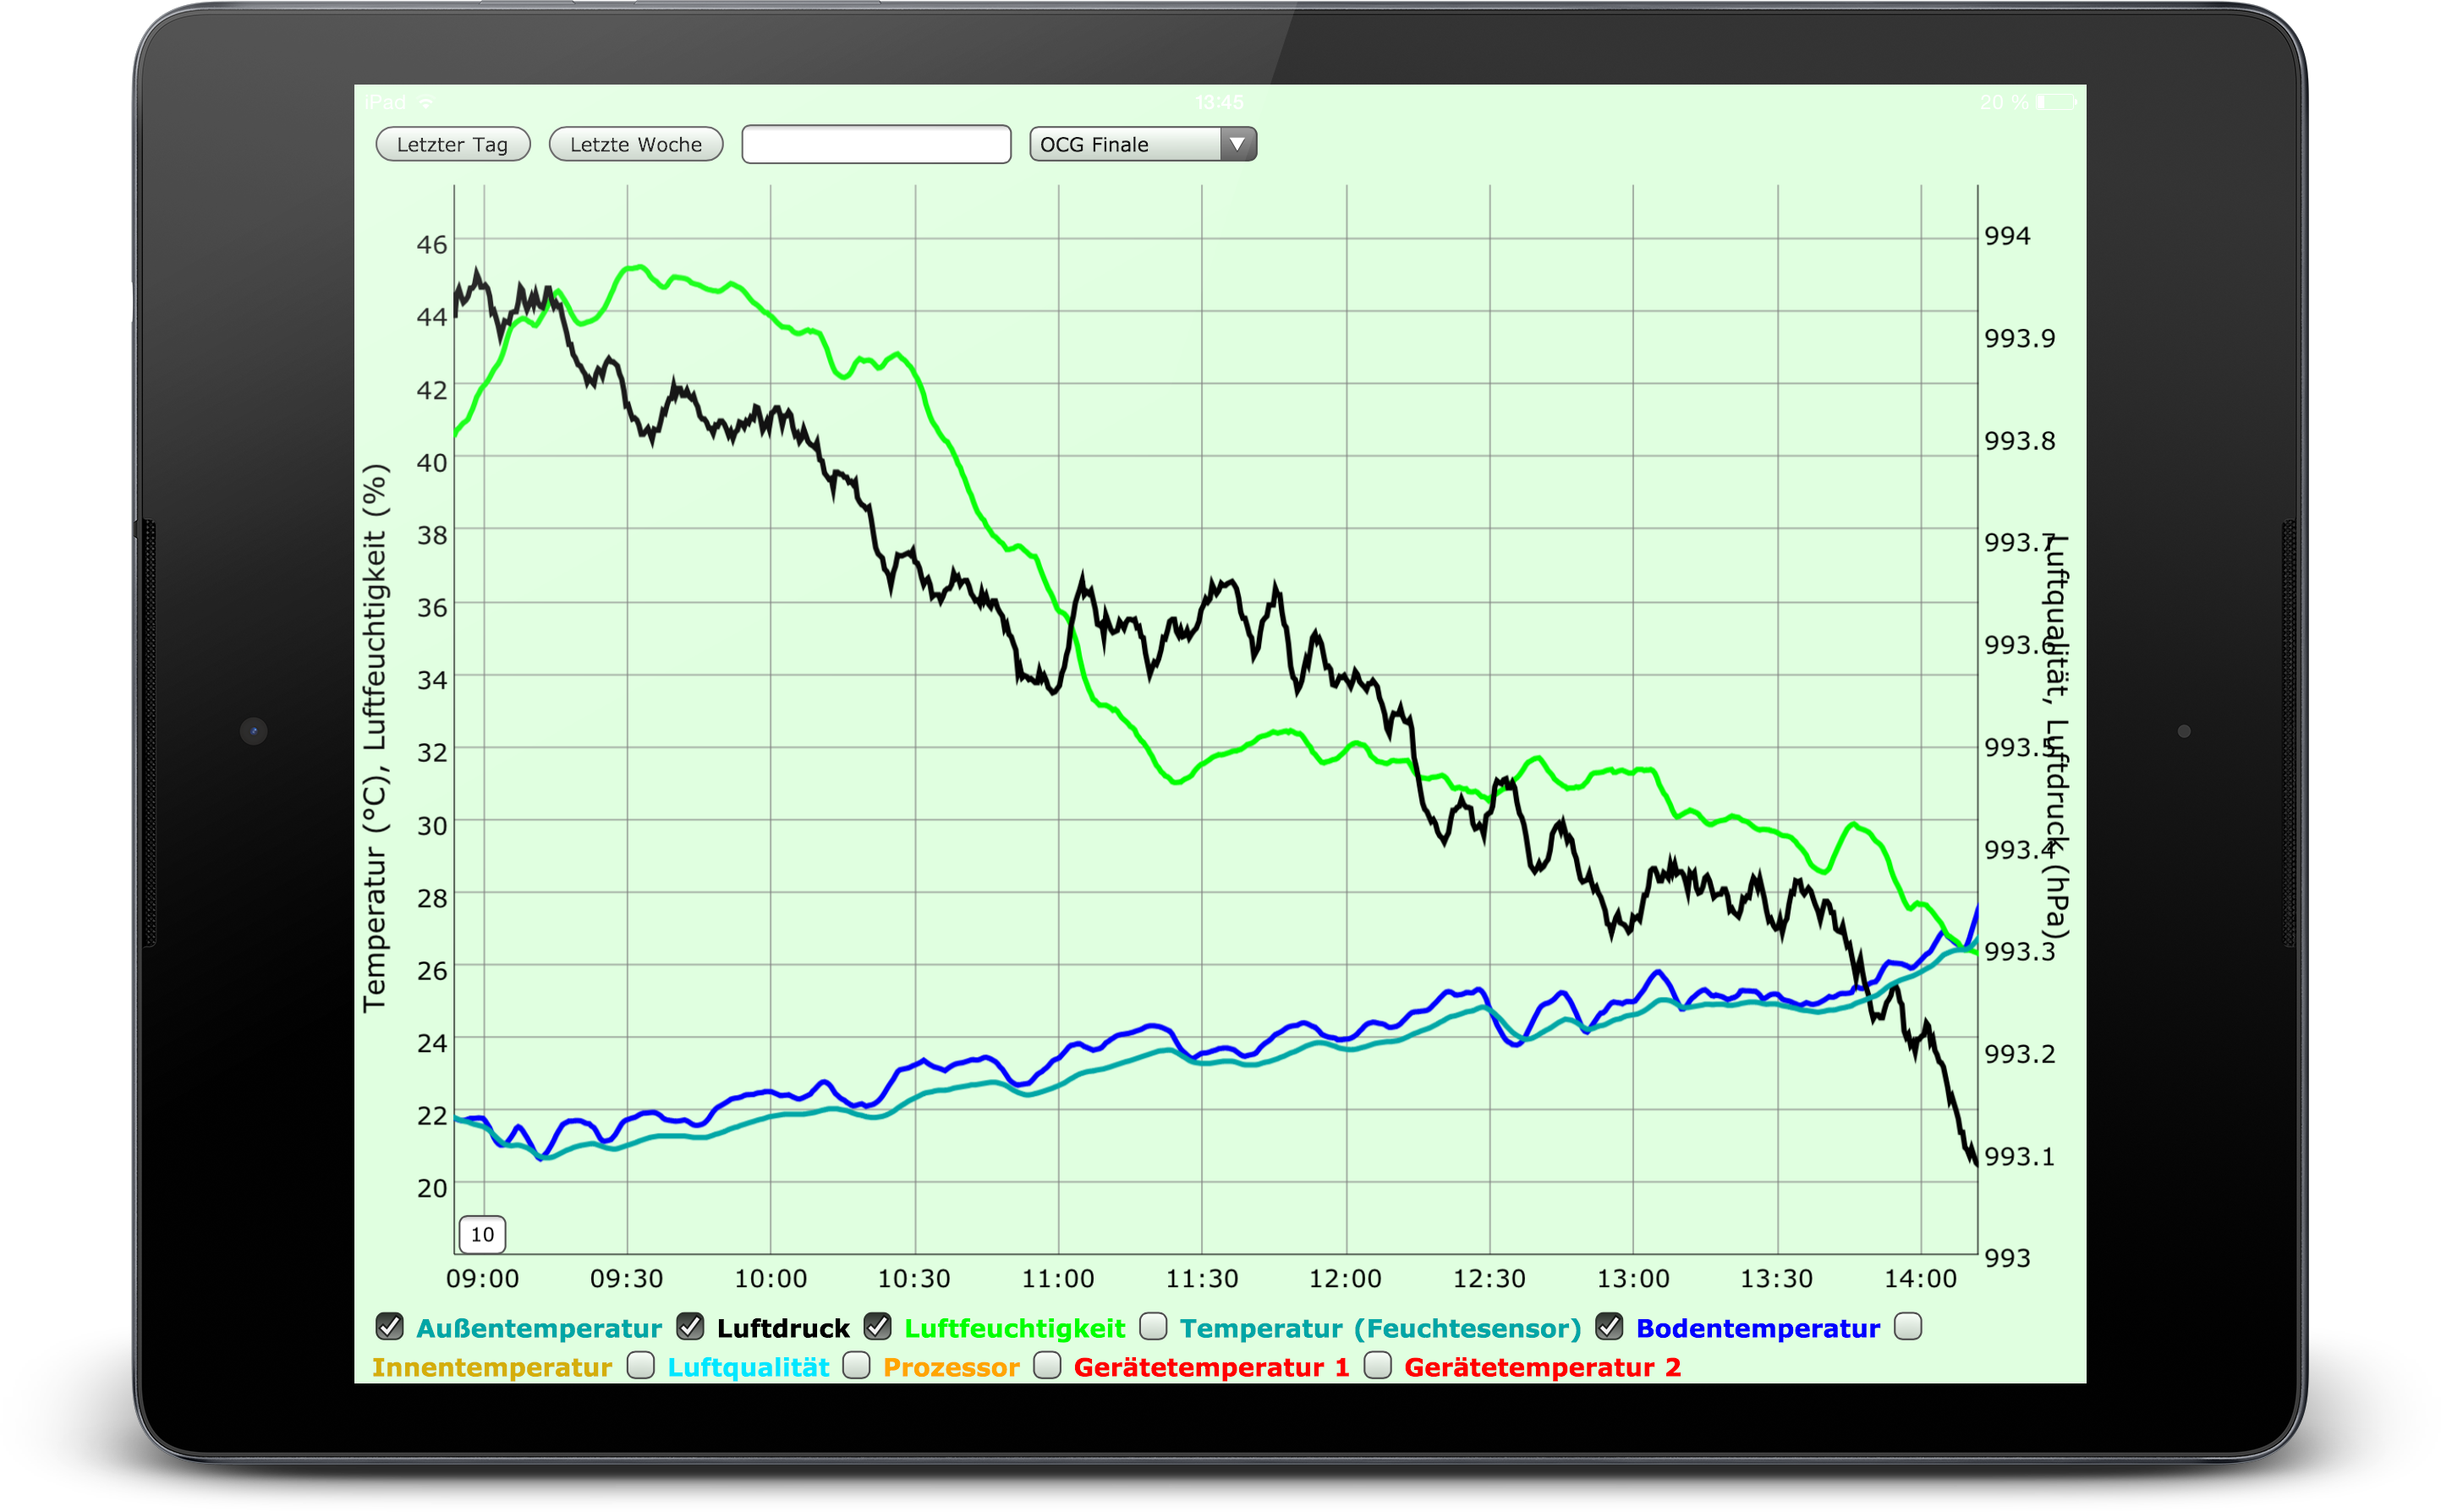
\includegraphics[width=1.35\textwidth]{figures/dygraphs_ipad.png}}
  \caption{Webinterface auf einem Tablet (eigenes Werk)}
  \label{fig:dygraphs_tablet}
\end{figure}

\begin{figure}[h]
  \centering
     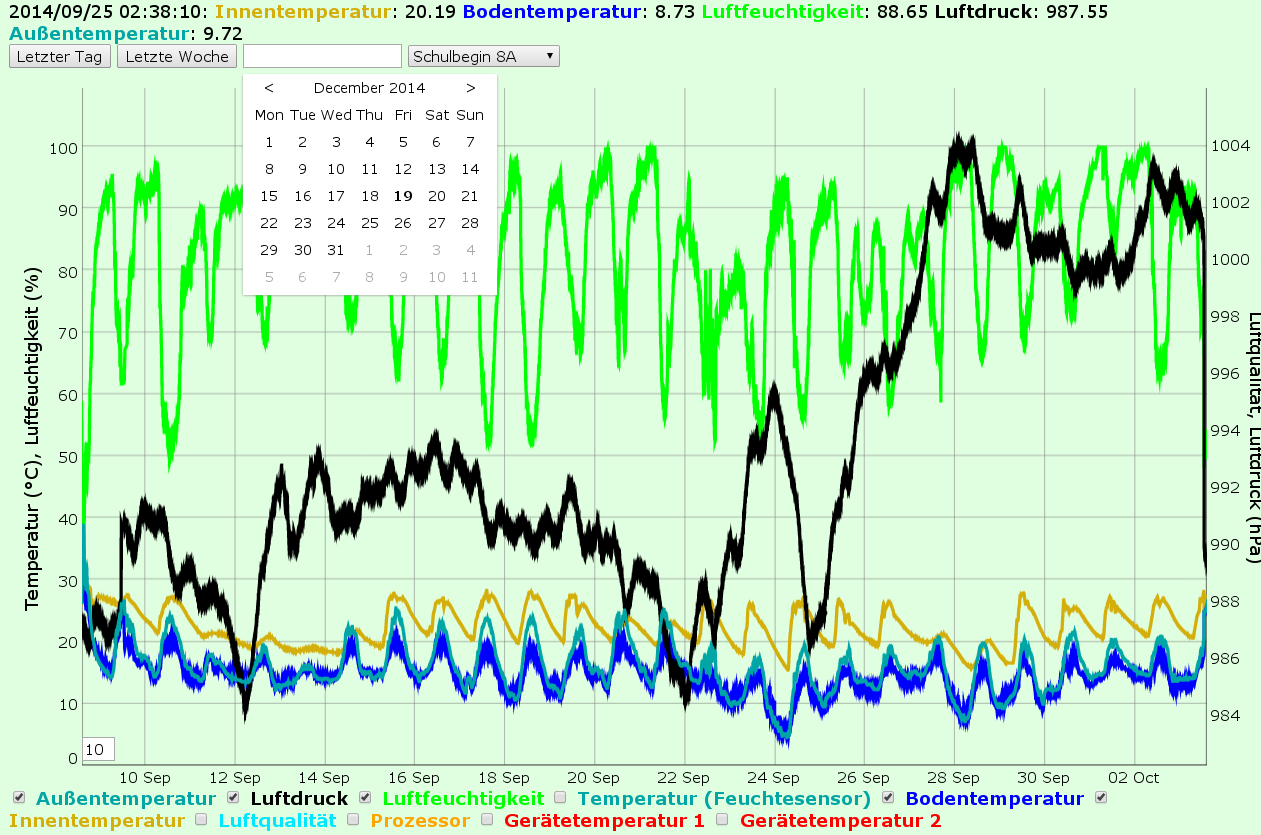
\includegraphics[width=\textwidth]{figures/dygraphs.png}
  \caption{Webinterface (von \href{http://winkler.kremszeile.at/dygraphs\_au\%C3\%9Fen.html}{winkler.kremszeile.at/dygraphs\_außen.html})}
  \label{fig:dygraphs}
\end{figure}
Damit auch die vergangenen Messergebnisse angesehen werden können, werden diese im Webinterface auf einer eigenen Seite als Diagramm dargestellt. Diese werden mithilfe von \emph{dygraphs}\footcite{dygraphs}, einer \gls{Javascript}-Bibliothek für interaktive Diagramme, erstellt.\footnote{\href{http://winkler.kremszeile.at/dygraphs_au\%C3\%9Fen.html}{winkler.kremszeile.at/dygraphs\_außen.html}}

Hierzu lädt der Webbrowser die komplette Aufzeichnung in Form der Datei \emph{dygraphs.csv} (siehe Datei \ref{file:dygraphs.csv}) nach. Daraus wird ein Diagramm über den gesamten Zeitraum der Messung erstellt. Im Gegensatz zu anderen Darstellungen kann hier jedoch einfach hineingezoomt werden. So können einfach einzelne Wochen oder Tage betrachtet werden. Da das Diagramm mit allen 10 Messkurven auf einmal überladen wäre, können einzelne Kurven aktiviert und deaktiviert werden. Zusätzlich kann ein Faktor eingegeben werden, um den die Kurven automatisch geglättet werden sollen. Mit einem Tastendruck kann man auch auf die letzten 24 Stunden oder 7 Tage zoomen oder in einem Kalender den Zeitraum auswählen. Es gibt auch ein Auswahlmenü, um den gewünschten Datensatz auszuwählen. Das Diagramm ist darauf angepasst, auch mit Tablets bzw. Touchscreens bedient zu werden.
Auf Youtube gibt es ein Video, wo man die Verwendung in Aktion sehen kann: \href{https://www.youtube.com/watch?v=1bv6CEXuN5c}{www.youtube.com/watch?v=1bv6CEXuN5c}

\section{Endauswertung}
\label{sec:Endauswertung}

Unabhängig vom Webinterface habe ich ein zweites Programm in \gls{Python} geschrieben. Dieses kann die fertige \emph{dygraphs.csv} (siehe Datei \ref{file:dygraphs.csv}) einlesen und verschiedene mathematische Auswertungen über einen beliebigen Zeitraum erstellen.

Zunächst wird die Datei in zwei Dateien aufgespalten. Die eine enthält nur die erste Spalte mit den Zeitstempeln jeder Messung, die andere die Messergebnisse. Da schon wenige Messfehler (zum Beispiel einmalig \SI{6}{\degreeCelsius} bei \SI{20}{\degreeCelsius} Außentemperatur) den Mittelwert (und die \gls{Standardabweichung}) stark verändern, wird zunächst nach Ausreißern gesucht. Hierzu wird für jeden Messwert überprüft, ob er um mehr als \SI{10}{\degreeCelsius} von dem vorherigen \emph{und} dem folgenden abweicht. Wenn dem so ist, wird eine Meldung ausgegeben:

\code{ausgabe.txt}{,morekeywords={Spalte,Zeile}}{5}{8}

Als nächstes kann man den Zeitraum angeben, für den die Auswertung erstellt werden soll. Zunächst wird überprüft, ob das eingegebene Datum gültig ist. Das Programm testet anschließend, welche Zeilen der Eingabedatei in diesem Zeitraum liegen.

\code{ausgabe.txt}{}{22}{28}

Nun werden für jede Spalte bzw. für jeden Sensor der Mittelwert, das Minimum, das Maximum und die \gls{Standardabweichung} berechnet und ausgegeben:

\code{ausgabe.txt}{}{29}{59}

\section{diverses}
\label{sec:diverses}

Abgesehen von den großen Teilen des Projektes gibt es auch einige kleinere Aspekte, von denen ich nun einige vorstellen möchte:

\subsection{Weather Underground}
\label{subsec:wunderground}

\emph{Weather Underground} ist ein Online-Wetterdienst mit Firmensitz in San Francisco.\footcite{wiki:wunderground} Dieser bietet auch die Möglichkeit eine eigene Wetterstation zu betreiben und die Daten auf ihrer Webseite anzuzeigen.\footnote{\href{http://www.wunderground.com/personal-weather-station/dashboard?ID=INIEDERS353}{www.wunderground.com/personal-weather-station/dashboard?ID=INIEDERS353}}
Leider werden die Wetterdaten nur in imperialen Einheiten (also \si{\degree F} und \si{\mmHg}\footnote{Millimeter-Quecksilbersäule oder Torr}) akzeptiert. Daher werden die Messwerte vorher von einem \gls{Python}-Programm umgerechnet und anschließend hochgeladen.

\subsection{Autostart}
\label{subsec:Autostart}

Damit die Umweltdatenmessung einfacher zu handhaben ist, gibt es ein einfaches Start-/Stop-Skript. So werden die Aufzeichnung und das Display automatisch beim Hochfahren gestartet und vor dem Herunterfahren ordnungsgemäß beendet.

\subsection{mitternacht.sh}
\label{subsec:mitternacht.sh}

Da der Raspberry Pi in der Schule hängt und nicht von außerhalb erreicht werden kann, ist es schwierig Softwareänderungen anzuwenden. Daher habe ich das kleine Skript \emph{mitternacht.sh} geschrieben. Dieses startet täglich um 0:00 Uhr und lädt die neuerste Version von \gls{Github} und installiert diese. Zusätzlich werden auch das Betriebssystem und alle installierten Programme aktualisiert. Anschließend werde ich per Push-Benachrichtigung über etwaige Probleme benachrichtigt und der Raspberry Pi startet neu.

\subsection{sonstiges}
\label{subsec:sonstiges}

\begin{itemize}
	\item ein Logo (siehe Abbildung \ref{fig:logo})
	\item Erstellung von statischen Diagrammen mit Gnuplot
	\begin{itemize}
		\item Jedoch bei zu vielen Daten unübersichtlich und langsam
	\end{itemize}
	\item Windows Vista/7 Gadget
	\item E-Mail und Push-Benachrichtigungen
	\item regelmäßiger Upload der Daten auf \href{http://winkler.kremszeile.at}{winkler.kremszeile.at}
\end{itemize}

\begin{figure}[h]
  \centering
     
\includegraphics[width=0.5\textwidth]{figures/logo.png}
  \caption{Logo (eigenes Werk)}
  \label{fig:logo}
\end{figure}